\chapter{The \LHCb experiment}
\label{chap:MoreStuff}

\chapterquote{Now, Now, There Will Be Plenty Of Time To Discuss Your Objections When And If You Return.}
{Professor Futurama}

\section{Energy Estimators}

% \begin{figure}
%   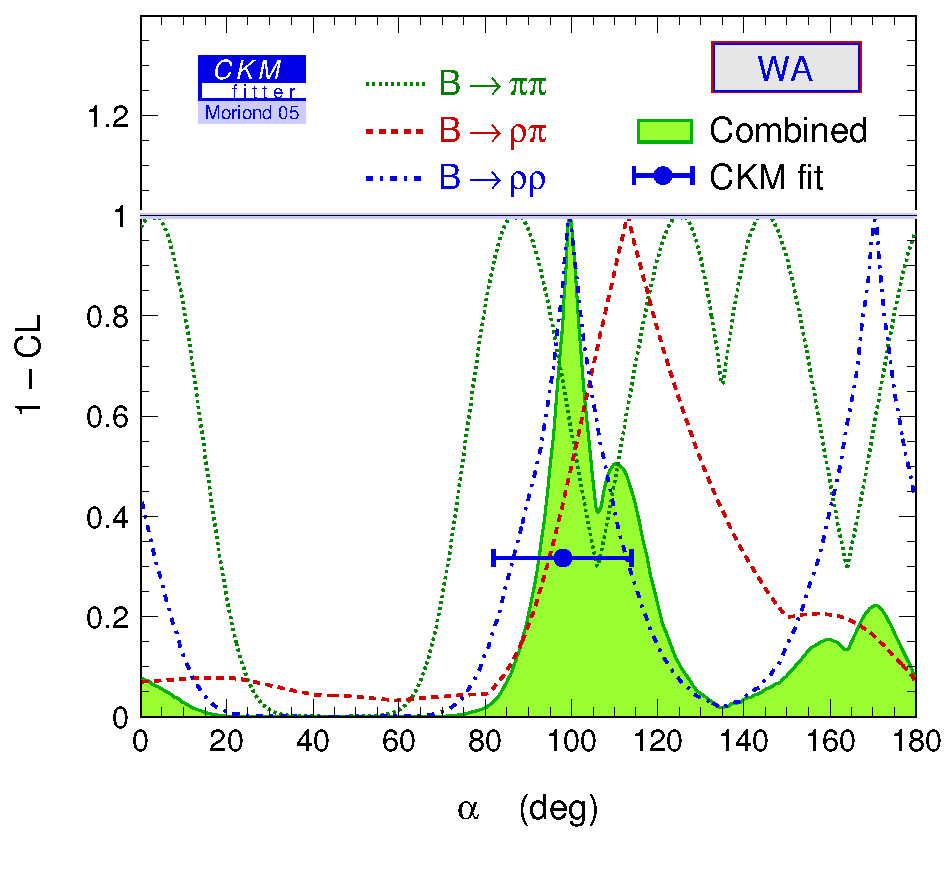
\includegraphics[width=\largefigwidth]{ckmfitter-alpha-combined}
%   \caption[CKM Fitter constraints on \alphaCKM.]%
%   {CKM Fitter constraints on \alphaCKM from combined \BToPiPi,
%     \BToRhoPi and \BToRhoRho decay analyses.}
%   \label{fig:CKMFitter}
% \end{figure}

\section{Energy Estimators in Particle Flow Calorimetry}
\label{sec:EnergyEstimatoresPFC}

In particle flow calorimetery the two methods of determining the energy of particles passing through the detector are calorimetric energy deposits and track fitting.  Due to the presence of a uniform magnetic field in the detector charged particles will bend and trace out a helix.  The radius of this helix will yeild the momenta of the charged particle in question and so the energy can be inferred assuming the mass of the particle is negligible in comparison to the momenta.

\begin{subequations}
  \label{eq:momentumApprox}
  \begin{equation}
    E^2 = | \mathbf{p} |^2 + m^2 \approx | \mathbf{p} |^2  
    \label{eq:momentumApprox1}
  \end{equation}
\end{subequations}


